\section*{Extended Data Fig. 1 | Sensitivity of each baseline to randomised residue assignment on DUD-E}

\begin{center}
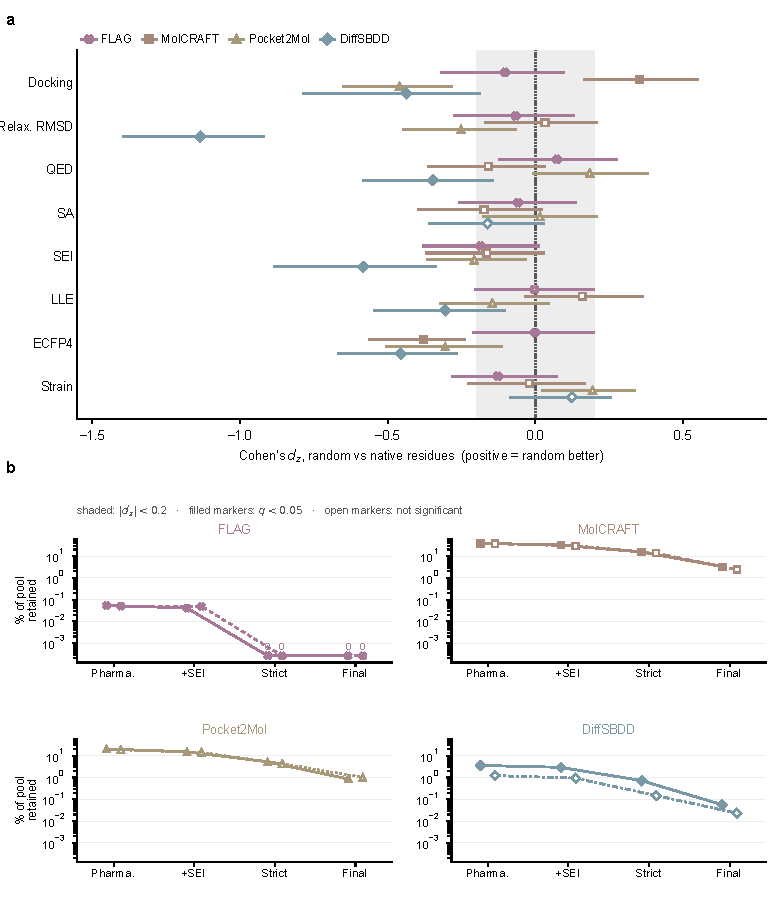
\includegraphics[width=131mm]{figures/si_fig_mapping_control.pdf}
\end{center}

\textbf{a}, Paired effect sizes (Cohen's $d_z$ with 95\% percentile intervals over targets) of the
random-residue arm against the native arm, for the four baselines that accept a residue-type
channel. Filled markers are significant after Benjamini--Hochberg correction across the eight
metrics of that method and open markers are not; the shaded band marks $|d_z|<0.2$. Positive values
mean the random arm scores better. \textbf{b}, Retention through the four-tier screening cascade as
a percentage of each arm's own generated pool, on a logarithmic scale, which makes methods with
different per-target budgets comparable. Solid lines and filled markers are the native arm, dashed
lines and open markers the random arm; a point at the axis floor labelled 0 means that no molecule
of that arm survived the tier. Each method pairs 96--102 DUD-E targets. DiffSBDD, FLAG and
Pocket2Mol were generated for this control at 300 molecules per target with both arms held to
identical per-target pools; MolCRAFT reuses an earlier campaign at about 1000 molecules per target,
whose two arms have unequal pools. GraphBP and ED2Mol take no residue-type input and are not shown.

Panel~\textbf{a} is tabulated in Extended Data Table~9.
